\documentclass[11pt]{article}
\def\shownotes{1}

\usepackage[top=3cm, bottom=3cm, left=2cm, right=2cm]{geometry}      % [top=2cm, bottom=2cm, left=2cm, right=2cm]
\geometry{letterpaper}                   % ... or a4paper or a5paper or ...
%\geometry{landscape}                % Activate for for rotated page geometry
%\usepackage[parfill]{parskip}
\usepackage{graphicx}
\usepackage{amssymb, amsmath, amsfonts}
\usepackage{amsthm}
\usepackage{enumerate}
\usepackage{hyperref}
\usepackage{xspace}
\usepackage{graphicx}
\usepackage{latexsym}
\usepackage{color}
\usepackage{framed}
\usepackage{algpseudocode}

\mathchardef\mhyphen="2D

\newcommand{\secref}[1]{\mbox{Section~\ref{#1}}}
\newcommand{\subsecref}[1]{\mbox{Subsection~\ref{#1}}}
\newcommand{\apref}[1]{\mbox{Appendix~\ref{#1}}}
\newcommand{\thref}[1]{\mbox{Theorem~\ref{#1}}}
\newcommand{\exref}[1]{\mbox{Example~\ref{#1}}}
\newcommand{\defref}[1]{\mbox{Definition~\ref{#1}}}
\newcommand{\corref}[1]{\mbox{Corollary~\ref{#1}}}
\newcommand{\lemref}[1]{\mbox{Lemma~\ref{#1}}}
\newcommand{\assref}[1]{\mbox{Assumption~\ref{#1}}}
\newcommand{\probref}[1]{\mbox{Problem~\ref{#1}}}
\newcommand{\clref}[1]{\mbox{Claim~\ref{#1}}}
\newcommand{\propref}[1]{\mbox{Proposition~\ref{#1}}}
\newcommand{\remref}[1]{\mbox{Remark~\ref{#1}}}
\newcommand{\consref}[1]{\mbox{Construction~\ref{#1}}}
\newcommand{\figref}[1]{\mbox{Figure~\ref{#1}}}
\DeclareMathOperator*{\expe}{\mathbb{E}}
\DeclareMathOperator*{\var}{\text{Var}}


\newcommand{\class}[1]{{\ensuremath{\mathsf{#1}}}}
\newcommand{\gen}{\ensuremath{\class{Gen}}\xspace}
\newcommand{\rep}{\ensuremath{\class{Rep}}\xspace}
\newcommand{\sketch}{\ensuremath{\class{SS}}\xspace}
\newcommand{\rec}{\ensuremath{\class{Rec}}\xspace}
\newcommand{\enc}{\ensuremath{\class{Enc}}\xspace}
\newcommand{\dec}{\ensuremath{\class{Dec}}\xspace}
\newcommand{\prg}{\ensuremath{\class{prg}}\xspace}
\newcommand{\zo}{\ensuremath{\{0, 1\}}}
\newcommand{\vect}[1]{\ensuremath{\mathbf{#1}}}
\newcommand{\zq}{\ensuremath{\mathbb{Z}_q}}
\newcommand{\Fq}{\ensuremath{\mathbb{F}_q}}
\newcommand{\sample}{\ensuremath{\class{Sample}}\xspace}
\newcommand{\neigh}{\ensuremath{\class{Neigh}}\xspace}
\newcommand{\dis}{\ensuremath{\mathsf{dis}}}
\newcommand{\decode}{\ensuremath{\mathsf{Decode}}}
\newcommand{\guess}{\mathsf{guess}}


\newcommand{\A}{\mathcal{A}}


\newcommand{\metric}{\ensuremath{\mathtt{Metric}}\xspace}
\newcommand{\hill}{\ensuremath{\mathtt{HILL}}\xspace}
\newcommand{\hillrlx}{\ensuremath{\mathtt{HILL\mhyphen rlx}}\xspace}
\newcommand{\yao}{\ensuremath{\mathtt{Yao}}\xspace}
\newcommand{\unp}{\ensuremath{\mathtt{unp}}\xspace}
\newcommand{\unprlx}{\ensuremath{\mathtt{unp\mhyphen rlx}}\xspace}
\newcommand{\metricstar}{\ensuremath{\mathtt{Metric}^*}\xspace}
\newcommand{\metricd}{\ensuremath{\mathtt{Metric}^*\mathtt{-d}}\xspace}
\newcommand{\hillstar}{\ensuremath{\mathtt{HILL}^*}\xspace}
\newcommand{\hillprime}{\ensuremath{\mathtt{HILL'}}\xspace}
\newcommand{\metricprime}{\ensuremath{\mathtt{Metric'}}\xspace}
\newcommand{\metricprimestar}{\ensuremath{\mathtt{Metric'}^*}\xspace}
\newcommand{\hillprimestar}{\ensuremath{\mathtt{HILL'}^*}\xspace}
\newcommand{\poly}{\ensuremath{\mathtt{poly}}\xspace}
\newcommand{\rank}{\ensuremath{\mathtt{rank}}\xspace}
\newcommand{\ngl}{\ensuremath{\mathtt{ngl}}\xspace}
\newcommand{\Hoo}{\mathrm{H}_\infty}
\newcommand{\Hav}{\tilde{\mathrm{H}}_\infty}
\newcommand{\Hfuzz}{\mathrm{H}^{\mathtt{fuzz}}_{t,\infty}}
\newcommand{\Huse}{\mathrm{H}_{\mathtt{usable}}}
\newcommand{\Dom}{\mathsl{Dom}}
\newcommand{\Range}{\mathsl{Rng}}
\newcommand{\Keys}{\mathsl{Keys}}
\def\col{\mathrm{Col}}

\newcommand{\ddetbin}{\ensuremath{\mathcal{D}^{det,\{0,1\}}}}
\newcommand{\drandbin}{\ensuremath{\mathcal{D}^{rand,\{0,1\}}}}
\newcommand{\ddetrange}{\ensuremath{\mathcal{D}^{det,[0,1]}}}
\newcommand{\drandrange}{\ensuremath{\mathcal{D}^{rand,[0,1]}}}

\newcommand{\expinfo}{\ensuremath{\mathcal{E}}}
\newcommand{\ext}{\ensuremath{\mathtt{ext}}}
\newcommand{\cext}{\ensuremath{\mathtt{cext}}}
\newcommand{\rext}{\ensuremath{\mathtt{rext}}}
\newcommand{\cons}{\ensuremath{\mathtt{cons}}}
\newcommand{\decons}{\ensuremath{\mathtt{decons}}}


\newcommand{\lwe}{\class{LWE}}
\newcommand{\LWE}{\class{LWE}}
\newcommand{\distLWE}{\ensuremath{\class{dist\mbox{-}LWE}}}

\newtheorem{theorem}{Theorem}[section]
\newtheorem{lemma}[theorem]{Lemma}
\newtheorem{proposition}[theorem]{Proposition}
\newtheorem{corollary}[theorem]{Corollary}
\newtheorem{definition}[theorem]{Definition}
\newtheorem{assumption}[theorem]{Assumption}
\newtheorem{claim}[theorem]{Claim}
\newtheorem{problem}[theorem]{Problem}
\newtheorem{construction}[theorem]{Construction}

\newcounter{ctr}
\newcounter{savectr}
\newcounter{ectr}

\newenvironment{newitemize}{%
\begin{list}{\mbox{}\hspace{5pt}$\bullet$\hfill}{\labelwidth=15pt%
\labelsep=5pt \leftmargin=20pt \topsep=3pt%
\setlength{\listparindent}{\saveparindent}%
\setlength{\parsep}{\saveparskip}%
\setlength{\itemsep}{3pt} }}{\end{list}}


\newenvironment{newenum}{%
\begin{list}{{\rm (\arabic{ctr})}\hfill}{\usecounter{ctr} \labelwidth=17pt%
\labelsep=5pt \leftmargin=22pt \topsep=3pt%
\setlength{\listparindent}{\saveparindent}%
\setlength{\parsep}{\saveparskip}%
\setlength{\itemsep}{2pt} }}{\end{list}}

\newenvironment{tiret}{%
\begin{list}{\hspace{2pt}\rule[0.5ex]{6pt}{1pt}\hfill}{\labelwidth=15pt%
\labelsep=3pt \leftmargin=22pt \topsep=3pt%
\setlength{\listparindent}{\saveparindent}%
\setlength{\parsep}{\saveparskip}%
\setlength{\itemsep}{2pt}}}{\end{list}}


\newenvironment{blocklist}{\begin{list}{}{\labelwidth=0pt%
\labelsep=0pt \leftmargin=0pt \topsep=10pt%
\setlength{\listparindent}{\saveparindent}%
\setlength{\parsep}{\saveparskip}%
\setlength{\itemsep}{20pt}}}{\end{list}}

\newenvironment{blocklistindented}{\begin{list}{}{\labelwidth=0pt%
\labelsep=30pt \leftmargin=30pt\topsep=5pt%
\setlength{\listparindent}{\saveparindent}%
\setlength{\parsep}{\saveparskip}%
\setlength{\itemsep}{10pt}}}{\end{list}}

\newenvironment{onelist}{%
\begin{list}{{\rm (\arabic{ctr})}\hfill}{\usecounter{ctr} \labelwidth=18pt%
\labelsep=7pt \leftmargin=25pt \topsep=2pt%
\setlength{\listparindent}{\saveparindent}%
\setlength{\parsep}{\saveparskip}%
\setlength{\itemsep}{2pt} }}{\end{list}}

\newenvironment{twolist}{%
\begin{list}{{\rm (\arabic{ctr}.\arabic{ectr})}%
\hfill}{\usecounter{ectr} \labelwidth=26pt%
\labelsep=7pt \leftmargin=33pt \topsep=2pt%
\setlength{\listparindent}{\saveparindent}%
\setlength{\parsep}{\saveparskip}%
\setlength{\itemsep}{2pt} }}{\end{list}}

\newenvironment{centerlist}{%
\begin{list}{\mbox{}}{\labelwidth=0pt%
\labelsep=0pt \leftmargin=0pt \topsep=10pt%
\setlength{\listparindent}{\saveparindent}%
\setlength{\parsep}{\saveparskip}%
\setlength{\itemsep}{10pt} }}{\end{list}}

\newenvironment{newcenter}[1]{\begin{centerlist}\centering%
\item #1}{\end{centerlist}}

\newenvironment{codecenter}[1]{\begin{small}\begin{centerlist}\centering%
\item #1}{\end{centerlist}\end{small}}

\ifnum\shownotes=1
\newcommand{\authnote}[2]{{\textcolor{red}{\textsf{#1 notes: }\textcolor{blue}{ #2}}\marginpar{\textcolor{red}{\textbf{!!!!!}}}}}
\else
\newcommand{\authnote}[2]{}
\fi
\newcommand{\bnote}[1]{{\authnote{Ben}{#1}}}
\newcommand{\lnote}[1]{{\authnote{Leo}{#1}}}
\newcommand{\rnote}[1]{{\authnote{Ran}{#1}}}
\newcommand{\onote}[1]{{\authnote{Omer}{#1}}}

\newcommand{\ve}{\vect{e}}
\newcommand{\vm}{\vect{m}}
\newcommand{\vy}{\vect{y}}
\newcommand{\vE}{\vect{E}}
\newcommand{\vS}{\vect{S}}
\newcommand{\vA}{\vect{A}}
\newcommand{\vc}{\vect{c}}
\newcommand{\vW}{\vect{W}}
\newcommand{\vQ}{\vect{Q}}
\newcommand{\vR}{\vect{R}}
\newcommand{\vU}{\vect{U}}
\newcommand{\vT}{\vect{T}}
\newcommand{\vX}{\vect{X}}
\newcommand{\vB}{\vect{B}}
\newcommand{\vz}{\vect{z}}
\newcommand{\vd}{\vect{d}}
\newcommand{\vs}{\vect{s}}
\newcommand{\vx}{\vect{x}}
\newcommand{\va}{\vect{a}}
\newcommand{\vb}{\vect{b}}
\newcommand{\vgamma}{\mathbf{\Gamma}}
\newcommand{\vt}{\vect{t}}
\newcommand{\vu}{\vect{u}}
\newcommand{\vF}{\vect{F}}
\newcommand{\recout}{x}
\newcommand{\ignore}[1]{}
\newcommand{\M}{\mathcal{M}}
\newcommand{\Vol}{\mathsf{Vol}}

\title{When are Fuzzy Extractors Possible?}


\begin{document}
\maketitle

\begin{abstract}
We characterize when deriving a stable key from a noisy source is possible.  We use the notation of fuzzy extractors introduced by Dodis et al. (Eurocrypt 2004).  The goal is to produce a strong $key$ from a $w$ drawn from a \emph{strong} distribution $W$ and to produce the same when given a nearby $w'$.  A fuzzy extractor is split into two algorithms $\gen$ which produces $key$ along with some helper information $p$ and $\rep$ which takes $w'$ and $p$ to reproduce $key$.  The key must remain strong in the presence of $p$.  The goal is to produce the correct key whenever $\dis(w, w')\le t$.

Ideally, key derivation should be possible whenever a negligible portion of $W$ lies within a ball~(arbitrarily centered) of radius $t$.  We call the maximum overall weight that lies within any ball of radius $t$ the fuzzy min-entropy of a distribution.  However, current techniques for constructing fuzzy extractors lie far from this necessary condition.  We investigate whether this is necessary for both fuzzy extractors and secure sketches~(a one round information-reconciliation component).  Our results are centered on feasibility and our constructions and impossibility results are primarily information-theoretic.
\end{abstract}

\section{Introduction}
Usually, authentication requires some high quality secret.  Traditionally, this secret is assumed to have high min-entropy.  However, many sources with sufficient entropy for authentication present an additional problem of noise.  That is, when the physical instantiation of the source is read multiple times, readings are close~(according to some metric) but not identical.  To use such sources in an authentication scheme it is often necessary to remove this noise and derive the same key from the initial and subsequent readings.

This problem was introduced in the seminal work of Bennett, Brassard, and Roberts~\cite{bennett1988privacy}.  They identify two fundamental tasks in noisy key derivation.  The first is known as information-reconciliation, removing the noise without leaking significant information, and the second is privacy amplification, converting the high entropy secret to a uniform random value.  In this work, we consider the non-interaction version of these problems where these tasks are performed non-interactively~(with a single message).

The paradigm for performing noisy key derivation using a single metric is known as fuzzy extractors~\cite{DBLP:journals/siamcomp/DodisORS08}.  Consider a particular high entropy distribution $W$.  Our goal is to derive stable keys from $W$ whenever the two readings~(denoted $w$ and $w'$ respectively) are within distance $t$.  A fuzzy extractor consists of two algorithms: generate~($\gen$) which takes the initial reading $w$ and produces $key$ along with a public helper value $p$.  The reproduce~($\rep$) algorithm takes the subsequent reading $w'$ along with the helper value $p$ to reproduce $key$.  The $key$ must be strong even to an adversary that has observed $p$~(the problem is trivial if $p$ is private).

Traditionally, fuzzy extractors are constructed by using a separate information-reconciliation component, known as a secure sketch, that maps $w'$ back to $w$ and a privacy-amplification component, a strong randomness extractor~\cite{nisan1993randomness}, that maps $w$ to a random key.  These objects can either be information-theoretic or computational.  The computational versions of these objects are defined in~\cite{krawczyk2010cryptographic} and~\cite{fuller2013computational} respectively.  Fuller et al.~\cite{fuller2013computational} show that computational secure sketches cannot improve significantly on information-theoretic secure sketches.

\textbf{A Necessary Condition:}  Intuitively, error-tolerance and key strength are at odds.  If the error-tolerance allows the entire metric space to authenticate then no security is possible.  As an example, consider a distribution $W$, where the adversary attempts to learn the key simply by inputting a point to the reproduce function.  Let $x^*$ be the point input by the adversary, the adversary learns the correct key whenever $\dis(w, x^*)\le t$.  For a fuzzy extractor to be secure this must occur with negligible probability.  That is, for all $x^*, \sum_{w\in W | \dis(w, x^*)\le t} \Pr[ W= w] \le \ngl(n)$.  We call the negative logarithm of this quantity the \emph{fuzzy min-entropy} of a distribution.  Clearly, the fuzzy min-entropy of a distribution must be super-logarithmic for any security.  Indeed, in the interactive setting this is a sufficient condition as well.  

However, in the one-round setting we are far from achieving security for all distributions with super-logarithmic fuzzy min-entropy.  Traditional fuzzy extractors and secure sketches incur at entropy loss of the size of the ball to be error-corrected.  While, this is optimal for the uniform distribution, it seems far from optimal for distributions where points are far apart.  Indeed, when the goal is provide key derivation from a source that has more errors than entropy, this bound provides no guarantee on the strength of the key.  The work of Canetti et al.~\cite{canetti2014key} shows it is possible to provide key derivation for some distributions of this type.  However, their work leaves the question open for a large number of distributions.  In this work, we attempt to settle this question: for what distributions is noisy key derivation possible and impossible?  \bnote{come back to this}

\textbf{Our results:} In this work we show awesome things!\bnote{write}

\section{Preliminaries}
\label{sec:preliminaries}
For a random variables $X_i$ over some alphabet $\mathcal{Z}$ we denote by $X = X_1,..., X_\ell$  the tuple $(X_1,\dots, X_\ell)$.  For a set of indices $J$, $X_{J}$ is the restriction of $X$ to the indices in $J$.  The set $J^c$ is the complement of $J$.  The {\em min-entropy} of $X$ is $\Hoo(X) = -\log(\max_x \Pr[X=x])$,
and the {\em average (conditional)} min-entropy of $X$ given $Y$ is  $\Hav(X|Y) = -\log(\expe_{y\in Y} \max_{x} \Pr[X=x|Y=y])$~\cite[Section 2.4]{DBLP:journals/siamcomp/DodisORS08}.   For a random variable $W$, let $H_0(W)$ be the logarithm of the size of the support of $W$,  that is $H_0(W) = \log |\{w | \Pr[W=w]>0\}|$.
The {\em statistical distance} between random variables $X$ and $Y$ with the same domain is $\Delta(X,Y) = \frac12 \sum_x |\Pr[X=x] - \Pr[Y=x]|$.
For a distinguisher $D$ we write the \emph{computational distance} between $X$ and $Y$ as $\delta^D(X,Y) = \left| \expe[D(X)]-\expe[D(Y)]\right |$ (we extend it to a class of distinguishers $\mathcal{D}$ by taking the maximum over all distinguishers $D\in\mathcal{D}$).  We denote by $\mathcal{D}_{s}$ the class of randomized circuits which output a single bit and have size at most $s$.

For a metric space $(\mathcal{M}, \dis)$, the \emph{(closed) ball of radius $t$ around $x$} is the set of all points within radius $t$, that is, $B_t(x) = \{y| \dis(x, y)\leq t\}$.  If the size of a ball in a metric space does not depend on $x$, we denote by $|B_t|$ the size of a ball of radius $t$.  We consider the Hamming metric over vectors in $\mathcal{Z}^\ell$, defined via $\dis(x,y) = \{i | x_i \neq y_i\}$.  For this metric, $|B_t| = \sum_{i=0}^t {\ell \choose i} (|\mathcal{Z}|-1)^i $.  $U_n$ denotes the uniformly  distributed random variable on $\{0,1\}^n$.  Unless otherwise noted logarithms are base $2$.
Usually, we use capitalized letters for random variables and corresponding lowercase letters for their samples.

\section{Fuzzy Extractors}\label{sec:fuzz extractor}

We now recall definitions and lemmas from the work of Dodis et. al.~\cite[Sections 2.5--4.1]{DBLP:journals/siamcomp/DodisORS08}, adapted to allow for a small probability of error, as discussed in \cite[Sections 8]{DBLP:journals/siamcomp/DodisORS08}.  Let $\mathcal{M}$ be a metric space with distance function $\dis$.

\begin{definition}
\label{def:fuzzy extractor}
An $(\mathcal{M}, m, \ell, t, \epsilon)$-\emph{fuzzy extractor} with error $\delta$ is a pair of randomized procedures, ``generate'' $(\gen)$ and ``reproduce'' $(\rep)$, with the following properties: 
\begin{enumerate}
\item The generate procedure \gen on input $w\in \mathcal{M}$ outputs an extracted string $r\in\{0,1\}^\ell$ and a helper string $p\in\{0,1\}^*$.
\item The reproduction procedure \rep takes an element $w'\in \mathcal{M}$ and a bit string $p\in\{0,1\}^*$ as inputs.  The \emph{correctness} property of fuzzy extractors guarantees that for $w$ and $w'$ such that $\dis(w,w')\leq t$, if $R,P$ were generated by $(R,P)\leftarrow\gen(w)$, then $\rep(w',P)=R$ with probability~(over the coins of $\gen, \rep$) at least $1-\delta$.  If $\dis(w,w')>t$, then no guarantee is provided about the output of \rep.
\item The \emph{security} property guarantees that for any distribution $W$ on $\mathcal{M}$ of min-entropy $m$, the string $R$ is nearly uniform even for those who observe $P$:  if $(R,P)\leftarrow\gen (W)$, then $\mathbf{SD}((R,P),(U_\ell,P))\leq \epsilon$.
\end{enumerate}
A fuzzy extractor is efficient if $\gen$ and $\rep$ run in expected polynomial time.
\end{definition}

Replacing the statistical distance in \defref{def:fuzzy extractor} with a computational distance results in a computational fuzzy extractor~\cite[Definition 2.5]{fuller2013computational}.

Secure sketches are the main technical tool in the construction of fuzzy extractors.  Secure sketches produce a string $s$ that does not decrease the entropy of $w$ too much, while allowing recovery of $w$ from a  close $w'$:
\begin{definition}
\label{def:secure sketch}
An $(\mathcal{M},m, \tilde{m}, t)$-\emph{secure sketch} with error $\delta$ is a pair of randomized procedures, ``sketch'' $(\sketch)$ and ``recover'' $(\rec)$, with the following properties:
\begin{enumerate}
\item The sketching procedure \sketch on input $w\in\mathcal{M}$ returns a bit string $s\in\{0,1\}^*$.
\item The recovery procedure \rec takes an element $w'\in\mathcal{M}$ and a bit string $s\in\{0,1\}^*$.  The \emph{correctness} property of secure sketches guarantees that if $\dis(w,w')\leq t$, then $\Pr[\rec(w',\sketch(w))=w]\geq 1-\delta$ where the probability is taken over the coins of $\sketch$ and $\rec$.  If $\dis(w,w')>t$, then no guarantee is provided about the output of \rec.
\item The \emph{security} property guarantees that for any distribution $W$ over $\mathcal{M}$ with min-entropy $m$, the value of $W$ can be recovered by the adversary who observes $w$ with probability no greater than $2^{-\tilde{m}}$.  That is, $\Hav(W|\sketch(W))\geq \tilde{m}$.
\end{enumerate}
A secure sketch is \emph{efficient} if \sketch and \rec run in expected polynomial time. 
\end{definition}

\textbf{Notes:} In the above definition of secure sketches (resp., fuzzy extractors), the errors are chosen before $s$ (resp., $P$) is known: if the error pattern between $w$ and $w'$ depends on the output of $\sketch$ (resp., $\gen$), then there is no guarantee about the probability of correctness.  Also we do not consider a computational version of secure sketches as Fuller et al. showed that computational secure sketches imply information-theoretic secure sketches with almost the same parameters~\cite[Corollary 3.8]{fuller2013computational}.


A fuzzy extractor can be produced from a \emph{secure sketch} and an \emph{average-case randomness extractor}. An average-case extractor is a generalization of a strong randomness extractor \cite[Definition 2]{nisan1993randomness}) (in particular, Vadhan~\cite[Problem 6.8]{Vad12} showed that all strong extractors are average-case extractors with a slight loss of parameters):
\begin{definition}
Let $\chi_1$, $\chi_2$ be finite sets.
A function $\ext: \chi_1\times \{0,1\}^d \rightarrow \{0,1\}^\ell$ a \emph{$(m, \epsilon)$-average-case extractor} if for all pairs
of random variables $X, Y$ over $\chi_1, \chi_2$ such that
$\tilde{H}_\infty(X|Y) \ge m$, we have $\Delta((\ext(X, U_d), U_d, Y), U_\ell\times
U_d \times Y) \le \epsilon$.
\end{definition}

\begin{lemma}
\label{lem:fuzzy ext construction}
Assume $(\sketch, \rec)$ is an $(\mathcal{M}, m, \tilde{m}, t)$-secure sketch with error $\delta$, and let $\ext:\mathcal{M}\times \zo^d \rightarrow \zo^\ell$ be a $(\tilde{m}, \epsilon)$-average-case extractor.  Then the following $(\gen, \rep)$ is an $(\mathcal{M}, m, \ell, t, \epsilon)$-fuzzy extractor with error $\delta$:
\begin{itemize}
\item $\gen(w):$ generate $x\leftarrow \zo^d$, set $p=(\sketch(w), x), r=\ext(w;x)$, and output $(r,p)$.
\item $\rep(w', (s, x)):$ recover $w=\rec(w',s)$ and output $r=\ext(w;x)$.
\end{itemize}
\end{lemma}

\subsection{A necessary condition for security}
\label{sec:minimal conditions}
We now define fuzzy min-entropy and show that fuzzy extractor security is only possible when the fuzzy min-entropy is super-logarithmic.



A necessary condition for fuzzy extractor security is that an adversary should not be able to learn the key simply by inputting a point into the \rep algorithm.  This means a negligible portion of the source distribution $W$ lies within any Hamming ball.  We make this intuition formal here:

\begin{definition}
\label{def:fuzzy min-ent}
A distribution $W$ in a metric space $(\mathcal{M}, \dis)$ has $(t, k)$-fuzzy min-entropy, denoted $\Hfuzz(W) \ge k$ if the following holds:
\[
\forall m\in \mathcal{M},  \sum_{w\in W | \dis(w, m)\le t} Pr[W=w] \leq 2^{-k}.
\]
\end{definition}
For a metric space $\mathcal{M}$, let $\max |\mathcal{M}|$ the maximum length required to describe an element $m\in\mathcal{M}$~(for most natural metric spaces this is $\log |\mathcal{M}|$).
\begin{lemma}
\label{lem:fuzz necessary}
Let $n$ be a security parameter and let $W$ be a distribution over $(\mathcal{M}, \dis)$.
If $\Hfuzz (W) = \Theta(\log n)$ there is no $(\mathcal{M}, W, \kappa, t)$-computational fuzzy extractor that is $(\max |\mathcal{M}| +  |\rep|, \epsilon)$-hard for $\epsilon = \ngl(n)$ with error $\delta = \ngl(n)$~(and thus no fuzzy extractor) for $\kappa =\omega(\log n)$.
\end{lemma}
\begin{proof}
Let $W$ be a distribution where $\Hfuzz(W) = \Theta(\log n)$.  This means that there exists a point $m\in \mathcal{M}$ such that $\Pr_{w\in W}[\dis (w, m)\leq t] \geq 1/\poly(n)$.  Consider the following distinguisher $D$:
\begin{itemize}
\item On input $r, p$.
\item If $\rep(m, p) = r$, output $1$.
\item Else output $0$.
\end{itemize}
First note that $|D|$ is of size $\max |\mathcal{M}|+ |\rep|$.  Clearly, $\Pr[D(R, P) = 1]\geq 1/\poly(n) - \delta$, while $\Pr[D(U_\kappa, P)=1 ]\leq 1/2^{-\kappa}$.  Thus, when $\kappa = \omega(\log n)$:
\[
\delta^D((R, P), (U_\kappa, P))\geq \frac{1}{\poly(n)} -\delta -  \frac{1}{2^{-\kappa}} = 1/\poly(n).
\]
\end{proof}
\lemref{lem:fuzz necessary} generalizes to interactive protocols, $D$ only provides an input to the protocol and looks at the output.  This means that fuzzy min-entropy is also a necessary condition for interactive solution.  In the interactive setting, fuzzy min-entropy is also a sufficient condition using secure two-party computation\bnote{cite something for this}.  However, in the non-interactive setting there are many distributions for which no construction is known to be secure and for which no impossibility result is known.  We attempt to bridge this gap in this work.

\section{Well-spread distributions}
In the remainder of this work, we consider increasingly complex types of distributions and consider both the minimum number of bits a secure sketch/fuzzy extractor must write down and the minimum entropy loss.  We begin by considering secure sketches.  We a call distribution well-spread if the distance between any two original readings $w_0, w_1$ is large.  Well-spread distributions should be the easiest type of distribution to handle as given a particular $w'$ there is a unique $w$ that could be the original reading.  Intuitively, no sketch should be necessary for such a distribution.  However, we show there is a large gap between a secure sketch that works for a particular well-spread distribution and a secure sketch that works for \emph{all} well-spread distributions.

\begin{table}
\begin{tabular}{l | l | c}
Upper bound & Depends on Distribution & Works for all Dist\\
\hline
Well-spread distribution & $0$ & $\log |B_t|$\\
Flat distribution & $\Hoo(W) - \Hfuzz(W) + \log (1/\delta)$ &$\log |B_t|$\\
Arbitrary distribution & $\Hoo(W) - \Hfuzz(W) + \log (1/\delta) + \log \log \mathcal{M}$ & $\log |B_t|$
\end{tabular}
\caption{Upper bounds on minimum number of bits that a fuzzy extractor can write down and still have recovery.}
\label{tab:upper bounds}
\end{table}
\subsection{Distribution Dependent Sketches}
Error-correction should be easy when all points of $W$ are far apart.  Intuitively, the fuzzy extractor/secure sketch does not need to disambiguate points and thus error-correction should be easy.  Indeed for any error-correcting code, a fuzzy extractor can be designed~(where the design of the fuzzy extractor depends on the supported distribution).  However, this intuition becomes more difficult when a fuzzy extractor should work for all well-spread distributions.  We begin by defining a well-spread distribution.

\begin{definition}
A distribution $W$ is called \emph{$t_{cor}$-well spread} if for all $w, x\in W, \dis(w, x)\ge t_{cor}$.
\end{definition}
Intuitively, it should be easy to build a fuzzy extractor for well-spread distributions when the desired error-tolerance is less than $t_{cor}/2$~(assuming the distribution has super-logarithmic min-entropy).  Indeed, this is the case when the fuzzy extractor is allowed to depend on $W$.

\begin{lemma}
\label{lem:nosketchwellspread}
Let $W$ be a $t_{cor}$ well-spread distribution with $\Hoo(W)\ge k$ there exists a $(\mathcal{M}, m, m, \lfloor( t_{cor}-1)/2\rfloor)$-secure sketch with no error that works for $W$.  In particular, $\sketch(w) = \perp$, and $\rec(w')$ finds the nearest $w\in W$.  \rec is efficient if there exists efficient decoding for the points in $W$.  By \lemref{lem:fuzzy ext construction} there also exists a $(\mathcal{M}, m,m -2\log 1/\epsilon, \lfloor (t_{cor}-1)/2\rfloor, \epsilon)$-fuzzy extractor with no error.
\end{lemma}  
\begin{proof}
It suffices to show that for any $w'$ there exists a unique $w\in W$ such that $\dis (w, w')\le \lfloor (t_{cor}-1)/2\rfloor$.  Since $W$ is $t_{cor}$-well spread, for all $w_0, w_1 \in W, \dis (w_0, w_1)\ge t_{cor}$.  Then by the triangle inequality,
\[
t_{cor}\ge \dis(w_0, w_1) \ge \dis(w_0, w') + \dis(w', w_1).\]
This is only true if at least one of $\dis(w_0, w')$ or $\dis(w', w_1)$ is greater than $\lfloor (t_{cor}-1)/2\rfloor$.
\end{proof}

\subsection{Distribution Agnostic Sketches}
Ideally, a fuzzy extractor should work for any distribution~(or at least a large family of distributions).  However, as we show below the above construction does not extend to the setting of all well-spread distributions.  In the previous model the particular well-spread distribution $W$ was encoded in the \sketch and \rec algorithms.  In this section we ask if a similar construction is possible when $(\sketch, \rec)$ must work for any well-spread distribution.  In this setting, $(\sketch, \rec)$ are described and the adversary then specifies a particular well-spread distribution $W$.

We show that any secure sketch that works for all well-spread distributions must write down a large number of bits~(matching our known constructions of secure sketches).  It is not known if it is necessary to decrease the entropy of the distribution $W$.

\begin{lemma}
Let $\mathcal{W}$ be the set of all $t_{cor}$-well spread distributions.  Let $t = \lfloor (t_{cor}-1)/2\rfloor$ and let $(\sketch, \rec)$ be a $(\mathcal{M}, m, \tilde{m}, t )$-secure sketch.  Then the length of $\sketch$ is at least $\log |B_{t}|$.
\end{lemma}
\begin{proof}
Let $\mathcal{M}$ be a metric space.
Let $\mathcal{W}$ be the set of all $t_{cor}$-well spread distributions on $\mathcal{M}$.  
Consider the following experiment:
\[
W\leftarrow \mathcal{W} \wedge w \leftarrow W \wedge w'\leftarrow B_{t_{cor}}(w) \wedge ss \leftarrow \sketch(w) \wedge w^* \leftarrow \rec(w', ss).
\]
That is, the adversary uniformly samples a well-spread distribution and then a point from the well-spread distribution.  
Since $(\sketch, \rec)$ works for any well-spread distribution the $\Pr[w^* = w] =1 $ in the above experiment.   Denote by $X$ the joint distribution of $w, w'$ produced in the above experiment.  Now consider the following experiment
\[
v \leftarrow U_{\mathcal{M}} \wedge v'\leftarrow B_{t_{cor}}(v) \wedge ss \leftarrow \sketch(v) \wedge v^* \leftarrow \rec(v', ss).
\]
Denote by $Y$ the joint distribution of $v, v'$ produced in the above experiment.  Then $X\overset{d}= Y$.  That is, the view of $(\sketch, \rec)$ is identically distributed in both cases.  Thus, $\Pr[v^* = v] = 1$.  For the uniform distribution the entropy retained by a secure sketch is at most $\Hav(U_{\mathcal{M}} | \sketch(U_{\mathcal{M}})) \le \log |\mathcal{M}| - \log |B_t(\cdot)|$~\cite[Lemma C.1]{DBLP:journals/siamcomp/DodisORS08}.  For a secure sketch to lose $\log |B_t(\cdot)|$ bits of entropy it must write down at least $\log |B_t(\cdot)|$ bits on average~\cite[Lemma 2.2b]{DBLP:journals/siamcomp/DodisORS08}.  Thus, $(\sketch, \rec)$ writes down at least $\log |B_t(\cdot)|$ bits on the uniform distribution and its view is identical on $X$ so it writes down at least $\log |B_{t_{cor}}|$ bits on $X$.  This completes the proof.
\end{proof}
\noindent
\textbf{Note:} In the above lemma, the relation between the well-spreadness of the class of distributions and the correctness of the fuzzy extractor is not important and is made to match the relation in \lemref{lem:nosketchwellspread} for convenience.  The bound is purely derived from the correctness condition, the well-spreadness of the distribution can essentially be arbitrarily replaced~(as long as the maximal distance point from any point in the metric space is the same).

Furthermore, the above lemma easily extends to the setting where the distributions are not well-spread as long as there is an adversary strategy of choosing the input distribution that produces an input to sketch that is identically distributed to the uniform distribution.

\section{Flat spread distributions}
In the previous section we showed bounds on producing secure sketches and fuzzy extractors for well-spread distributions.  In this section we further investigate secure sketches where the sketch depends on the input distribution.\footnote{Recall the bound when the sketch does not know the input distribution is $\log |B_t|$ bits and this is constructible for any distribution.}

\subsection{Distribution Dependent Sketches}

\lemref{lem:nosketchwellspread} showed that if a fuzzy extractor~(resp. secure sketch) is built for a particular well-spread distribution, it is not necessary to write down information-reconciliation information.  In this section, we consider information-theoretic bounds on distributions that contain multiple points in each ball.  
We begin by considering flat distributions where the probability of each point in $W$ is the same.

\begin{definition}
A distribution $W$ is \emph{flat} if for all $w_0, w_1 \in W$, $\Pr[W=w_0] = \Pr[W=w_1]$.  
\end{definition}

Recall that fuzzy min-entropy is a lower bound of the adversaries success probability for any scheme~(\defref{def:fuzzy min-ent}).  Fuzzy min-entropy is total weight of the maximum probability ball.  For flat distribution, this is directly correlated to the ball with the largest number of points.  That is, for a flat distribution 
\begin{align*}
\Hfuzz(W) &= -\log \max_{w^* \in \mathcal{M}} \{w | w\in W \wedge \dis(w, w^*)\le t\} * \Pr[W=w]\\
&= -\log \max_{w^* \in \mathcal{M}} \{w | w\in W \wedge \dis(w, w^*)\le t\} *2^{-\Hoo(W)}\\
&=\Hoo(W) -\log \max_{w^* \in \mathcal{M}} \{w | w\in W \wedge \dis(w, w^*)\le t\} 
\end{align*}
For notational convenience, we denote the ball with the largest number of points as $B_{t, max}$.  For any scheme, the adversary's success probability is 
\begin{align}
\Hfuzz(W) = \Hoo(W) -\log |B_{t, max}|.\label{eq:fuzz for flat}
\end{align}
%We start by considering distributions that have a fixed number of neighbors for each point.
%
%\begin{definition}
%We call a distribution $W$, over metric space $\mathcal{M}$, $(c, t)$-\emph{fixed neighbor} if there exists a constant $c$ such that for all points in $x\in \mathcal{M}$ there are exactly $c$ points $w\in W$ such that $\dis(w, x)\le t$.  We say that $W$ is a $(c, t)$-\emph{bounded neighbor distribution} if for all point $x\in\mathcal{M}$ there are at most $c$ points $w\in W$ such that $\dis(w, x)\le t$.
%\end{definition}
%
%\textbf{Note:} A fixed neighbor distribution is a special case of a bounded-neighbor distribution.
We now present an information-theoretic construction for flat distributions.  We first introduce the notion of a pairwise-independent hash:

\begin{definition}
Let $F : \mathcal{K} \times D \to R$ be a function.  We say that $F$ is \emph{universal} if for all distinct $x_1, x_2 \in D$:
\[
 \Pr_{K \leftarrow \mathcal{K}}[F(K, x_1) = F(K, x_2)] = \frac{1}{|R|} \;.
\]
%In other words, $F(K,x_1),F(K,x_2)$ are all uniformly and independently random over $R$. 
\end{definition}

We now show a sufficiently-long universal hash function suffices to construct an information-theoretic fuzzy extractor.

\begin{construction}
\label{cons:pairwise hash}
Let $W$ be a flat distribution over $\mathcal{M}$.  Let $F :\mathcal{K}\times \mathcal{M}\rightarrow R$ be a pairwise independent hash function.  We describe $\sketch, \rec$ as follows:
\begin{itemize}
\item $\sketch(w)$:
\subitem Sample $K\leftarrow \mathcal{K}$.
\subitem Set $p = F(K, w), K$.
\item $\rec(w', y, K)$:
\subitem Enumerate $W^* = \{w \in W | \dis(w, w')\le t\}$.
\subitem For all $w^*\in W^*$, if $F(K, w^*) = y$, output $w^*$.
\subitem Output $\perp$.
\end{itemize}
\end{construction}
\begin{lemma}
\consref{cons:pairwise hash} is a $(\mathcal{M}, m, m - \log |R|, t)$-secure sketch with error $\delta \le \frac{|B_{t, max}|-1}{|R|}$. 
\end{lemma}
\begin{proof}
We first argue security.  Since $\mathcal{K}$ and $W$ are independent $\Hav(W | \mathcal{K}) = \Hoo(W) = m$.  Then by \cite[Lemma 2.2b]{DBLP:journals/siamcomp/DodisORS08}, $\Hav(W | \mathcal{K}, F(K, W)) \ge \Hoo(W) - \log |F(K, W)| \ge m - \log |R|$.

We now argue correctness.  Fix some $w, w'$.  Let $W^*$ denote the set of elements in $W$ within distance $t$ of $w'$ recall that the size of $W^*$ is at most $B_{t, max}$ and since $w, w'$ are chosen independently of $\sketch$ this set is independent of the choice of $\mathcal{K}$.  Note $\rec$ will never output $\perp$ as the correct $w$ will match the hash, our goal is to bound the probability that another element $w^*$ collides, that is $F(K, w^*) = F(K, w)$.
\begin{align*}
\Pr[\exists w^* \in W^* |w^* \neq w \wedge F(K, w^*) = F(K, w)] &\le \sum_{w^*\in W^* | w^*\neq w} \Pr[F(K, w^*) = F(K, w)] \\
 &= \sum_{w^*\in W^* | w^*\neq w} \frac{1}{|R|} = \frac{|B_{t, max}|-1}{|R|}
\end{align*}
Where the inequality proceeds by union bound, the first equality proceeds by the universality of $F$, and the second equality proceeds by noting the number of neighbors is bounded by $|B_{t, max}|$.  This completes the proof.
\end{proof}
\begin{corollary}
Let $n$ be a security parameter.  
If $|R| \ge |B_{t, max}|* n^{\omega(1)}$ then \consref{cons:pairwise hash} is correct with overwhelming probability.  That is, setting $\log |R| = \log |B_{t, max}| + \omega(\log n)$ suffices.
\end{corollary}

Note that \consref{cons:pairwise hash} writes down essentially the worst case number of bits in all setting, it knows the maximum number of points in any ball and writes down that number~(with an additional super-logarithmic factor to prevent collisions).  Recall, our hope is to find a sketch that achieves total security equal to the fuzzy min-entropy of the distribution.  Thus, the remaining entropy for this construction is 
\[
\Hav(W |\sketch(W)) = \Hoo(W) - \log |B_{t, max}| - \omega(\log n)
\]
For a flat distribution this is within a super-logarithmic factor of optimal~(see Equation~\eqref{eq:fuzz for flat}).  Intuitively, this is because the sketch is deconflicting for the ball with the largest number of points.  For a flat distribution, this is also the ball with the largest total weight.  We will see this becomes more difficult as we move to the setting where points have very different probability.  In this setting, we may write down a large number of bits to deal with a low weight ball that has a large number of points, but this may completely reveal the high weight balls. We will compensate for this problem by writing down a variable number of bits.
%with a fixed number of neighbors, 
%\begin{align*}
%\Hfuzz(W) &= -\log \max_{x\in \mathcal{M}}, \sum_{w | \dis(w, x)\le t} \Pr[W=w]\\
%&=-\log \max_{x\in \mathcal{M}}, -\log \sum_{w | \dis(w, x)\le t} 2^{-\Hoo(W)}\\
%&= -\log c2^{-\Hoo(W)} = \Hoo(W) - \log c
%\end{align*}
%Thus, the construction is optimal up to a super-logarithmic factor for flat sources with a fixed number of neighbors.  We now attempt to remove both of these restrictions.


\bnote{need to extend this to a non-fixed number of bits and randomized.}
\section{Dealing with non flat distributions}
The hashing approach outlined above~(\consref{cons:pairwise hash}) does not extend to arbitrary sources.  The reason is that some balls may have significantly more points but low overall probability.  Let $W$ be a distribution, denote by $B_1$ a ball with $2^{\Hoo(W)}$ points but with probability $\Pr[W\in B_1] =2^{-\Hoo(W)}$ and let $B_2,..., B_{2^{-\Hoo(W)}}$ be well-spread balls with one point each with probability $\Pr[W\in B_i] = 2^{-\Hoo(W)}$.  Then the hashing algorithm outlined above it is necessary to write down $\Hoo(W)$ bits in the case when $W$ lands in $B_1$.  However, with probability $1-2^{-\Hoo(W)}$ the point $w_0$ lies outside of $B_1$ and the hash may completely reveal the point in this setting.  

Dealing with non-flat distributions requires a new strategy.  Ideally, this strategy should be aware of the density of the current ball and aware that when an original reading comes from a sparse ball it is not necessary to write down many bits.  We first a natural method to leverage convex combinations that does not work\bnote{phrasing}.  We then show a solution that comes within \bnote{something} of optimal by partitioning the probability space.

\subsection{Leveraging convex combinations?}
In many situations solving a problem for min-entropy distributions can be reduced to solving the problem for flat distributions and then using the fact that any min-entropy distribution is a convex combination of flat distributions.  For example, consider the following extension to \consref{cons:pairwise hash}.  Let $W$ be some distribution that is a finite convex combination of flat sources $W_1,..., W_n$ where each $\forall i, \Hoo(W_i)\ge k$.\footnote{A distribution may be an  convex combination of an infinite number of distributions.  However, we show it is difficult to leverage convex combinations in the finite setting and handling the infinite case is more difficult.}  For convenience we assume that the coefficients on all $W_i$ are the same and distributions may be repeated. 

The proposed modification to the construction is as follows, when receiving an input $w$, sample a distribution $W_i$ from the set of distributions where $w$ has nonzero probability, then write down $i$ and perform the sketch as before for distribution $W_i$.  Intuitively, writing down a distribution $i$ should not do any harm as each of distributions $W_i$ has the same min-entropy as the starting distribution.  Furthermore, each of these distributions is flat and thus, \consref{cons:pairwise hash} should apply.

In the flat case, we saw it was necessary to write down the number of points in the largest ball, however, the residual entropy in this case was exactly equal to the density of the largest ball~(matching the success of the best adversary that always guesses in this ball).  That is, the residual entropy $\Hav(W|\sketch(W)) \approx \Hfuzz(W)$.  However, in the setting where $W$ is a convex combination of flat sources this does not hold.

Consider set of distributions $W_i$ where each $W_i$ has two components, first $W_i$ contains a distinguished point $w^*$ where $\Pr[W=w^*] = 2^{-k}$ and $w^*$ has no neighbors, second let $W_i$ contain a set $B_i$ of $2^{-k}-1$ points within distance $t$ each with probability $2^{-k}$.  This distribution is illustrated in \figref{fig:convex comb}.  

The fuzzy min-entropy of $W_i$ is almost $0$ as the overwhelming majority of the probability space lies in $B_i$.  Now consider the distribution $W$ that is a convex combination of the $W_i$~(we assume that $B_i$ do not intersect).  Note that $\Hoo(W)=k$ and that $\Hfuzz(W)\approx \min\{\ell, k\}$ where $\ell$ is the number of distributions $W_1,..., W_\ell$.  (For our purposes, we can assume that $\ell$ is quite large and the probability of $w^*$ becomes the dominant factor.)

Consider an input point $w\in W$.  One of two cases occurs either $w=w^*$ or $w\in B_i$ for some $i$.  It should be clear in either case that the selected distribution $W_i$ is uniformly distributed from $\{1,..., \ell\}$.  For any of the selected distributions, there is a ball with $\approx 2^{-k}$ points and thus the hash based construction must write down approximately $k$ points.  This means that $\Hav(W | \sketch(W))  = \Hav(W_i | \sketch(W_i)) \approx 0$.  This is despite the fact $\Hfuzz(W) \approx \min\{\ell, k\}$.  Thus, the ability to sketch flat distributions does not easily admit a technique to sketch non-flat distributions.  In the following discussion, we present a more complicated technique that layers the distribution to make it appear flat.

\begin{figure}[h]

\centering
    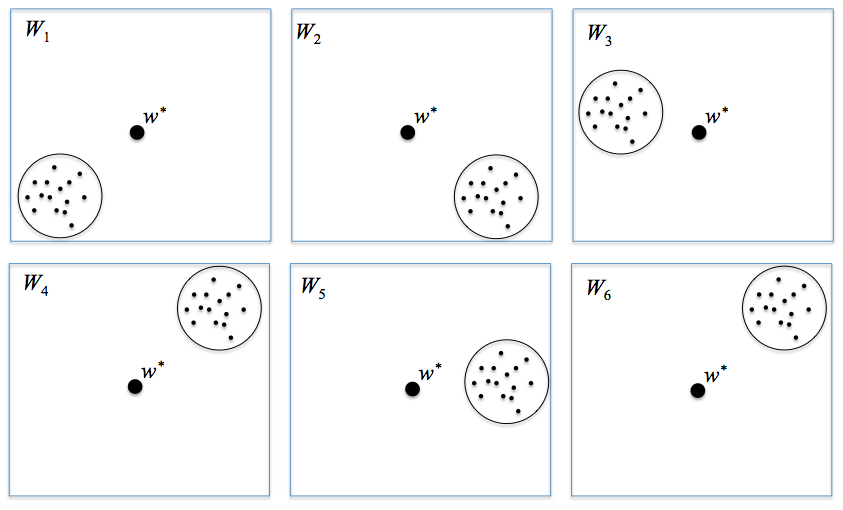
\includegraphics[width=.9\textwidth]{convexCombExample.png}
    \caption{A convex combination of $W_1,..., W_\ell$ has high min and fuzzy min-entropy, but sketching by using the component flat distributions removes all entropy.}
\label{fig:convex comb}    
\end{figure}

\bnote{remove pagebreak later}

\subsection{Layered Hashing}
As we saw in the previous section, dealing with non-flat distributions is difficult.  The problem is distinguishing between the setting where a ball has a few high probability points and a large number of low probability points.  We will deal with this problem by describing the probability of the point $w_0\in W$ seen in sketch.  Then the hash is applied only considering the maximum weight of the ball containing points at this level.  Roughly, at each layer we can think of the distribution as being flat, and the only additional information is the layer of the original reading.

\pagebreak

\begin{construction}
\label{cons:leveling}
Let $\mathcal{M}$ be a metric space and let $n =\log |\mathcal{M}|$.  Let $\Hoo(W) \ge m$
Let $\ell\in\mathbb{Z}^+$ be a parameter.  Let $L_i = (2^{-(i+1)}, 2^{-i}]$ for $i=m,..., n+\ell$.  Let $F_i :\mathcal{K}_i\times \mathcal{M}\rightarrow R_i$ be a parameterized family of pairwise independent hash functions.  We describe $\sketch, \rec$ as follows:
\begin{itemize}
\item $\sketch(w)$:
\subitem If $\Pr[W=w]\le 2^{-(n+\ell)}$
\begin{itemize}
\item Set $p=0, w$.
\end{itemize}
\subitem Else
\begin{itemize}
\item Find $i$ such that $\Pr[W=w]\in L_i$.  
\item Sample $K\leftarrow \mathcal{K}_i$.
\item Set $p =1,  i, F_i(K, w), K$.
\end{itemize}
\item $\rec(w', y)$:
\subitem If $y_0 = 1$, output $y_{1,..., |y|}$.
\subitem Else parse $(i, z, K) = y_{1,..., |y|}$.
\subitem Enumerate $W^* = \{w \in W | \dis(w, w')\le t\}$.
\subitem For all $w^*\in W^*$, if $F(K, w^*) = z$, output $w^*$.
\subitem Output $\perp$.
\end{itemize}
\end{construction}

Before describing the bounds obtained by \consref{cons:leveling} we will extend our notation for the maximum likelihood ball to the leveled case.  Let $B_{t, i, max}$ be the ball that contains the most points in $L_i$.  That is,
\[
B_{t, i, max} = \max_{w^* \in \mathcal{M}} \{w | w\in W \wedge \dis(w, w^*)\le t \wedge \Pr[W=w]\in L_i\}.
\]
\begin{theorem}
Let $\delta>0$ be an function of $n$.  Let $F_i: \mathcal{K}_i \times \mathcal{M}\rightarrow R_i$ be a parameterized family of pairwise independent hash functions where $|R_i| = |B_{t, i, max}| /\delta$.  Then \consref{cons:leveling} is a $(\mathcal{M}, m, \tilde{m}, t)$-secure sketch with error $\delta$ for $\tilde{m} = \Hfuzz(W) - \log n - \log 1/\delta - 3$.
\end{theorem}
\bnote{right now this is stated without $\ell$.  I found the expression to be really gross with $\ell$ included.  Thoughts?  I know $\ell$ needs to be there because the construction uses it.}
\begin{proof}
We begin by arguing correctness.  Fix some $w, w'$.  If $\Pr[W=w]\le 2^{-(n+\ell)}$, then $w$ is simply transmitted to $\rec$ and correctness is trivial.  Now consider the case when $\Pr[W=w]> 2^{-(n+\ell)}$, let $L_i^*$ be the level of $\Pr[W=w]$.
Let $W^*$ denote the set of elements in $W$ within distance $t$ of $w'$ such that $\forall w \in W^*, \Pr[W^*=w]\in L_i^*$. The size of $W^*$ is at most $B_{t, i, max}$. The choice of $w, w'$ is independent of $\sketch$, so this set is independent of $\mathcal{K}_i$~(it does effect the value of $i$ but not the particular outcome from $\mathcal{K}_i$).  Note $\rec$ will never output $\perp$ as the correct $w$ will match the hash.  The probability that another element $w^*$ is:
\begin{align*}
\Pr[\exists w^* \in W^* |w^* \neq w \wedge F(K, w^*) = F(K, w)] &\le \sum_{w^*\in W^* | w^*\neq w} \Pr[F(K, w^*) = F(K, w)] \\
 &= \sum_{w^*\in W^* | w^*\neq w} \frac{1}{|R_i|} = \frac{|B_{t, i, max}|-1}{|R_i|} = \delta
\end{align*}
Where the inequality proceeds by union bound, the first equality proceeds by the universality of $F$, and the second equality proceeds by noting the number of neighbors is bounded by $|B_{t, i, max}|$.  

We now argue security.  First note that the total weight of points whose probability is less than $2^{-(n+\ell)}$ is at most $2^{-\ell}$~(there are at most $2^n$ points in the distribution).  That is, $\sum_{w | \Pr[W=w]\le 2^{-(n+\ell)}}\Pr[W = w] \le 2^{-\ell}$.  Let $1_{\text{low prob}}$ be the indicator random variable for $\Pr[W=w]\le 2^{-n}$.  Then 
\begin{align*}
\Hav(W | \sketch(W)) = -\log \left(\Pr[1_{\text{low prob}}=1] * 1 + \Pr[1_{\text{low prob}} =0]   2^{-\Hav(W | \sketch(W) \wedge 1_{\text{low prob}} = 0)}\right)\\
-\log\left( 2^{-\ell} + (1-2^{-\ell})2^{-\Hav(W | \sketch(W) \wedge 1_{\text{low prob}} = 0)}\right)
\end{align*}
We first consider the optimum strategy for an adversary that receives just the information about the probability of $w$.  An adversary that receives $i$ as input the best strategy is to guess a point that has the most nearby weight in that layer.  That is, $w^*\leftarrow A(i)$ such that $\max_{w^* \in \mathcal{M}}\Pr_{w\in W | 2^{-(i+1)}\le \Pr[W=w]\le 2^{-i}}[\dis(w, w^*)]$.The success of this adversary is at least $2^{-(i+1)}|B_{t,i, max}|$ as there at $B_{t, i, max}$ nearby points in that layer each with probability at least $2^{-(i+1)}$.  Note there are $n-m+\ell$ outcomes for $i$ so the overall success of such an adversary is at most $n-m+\ell$ better than an adversary without such input~(by~\cite[Lemma 2.2]{DBLP:journals/siamcomp/DodisORS08}).  That is, 
\begin{align}
\expe_{i | m\le i \le n+\ell}2^{-(i+1)}|B_{t, i, max}|&\le \expe_{i | m\le i \le n+\ell}\left( \max_{w^*\in W}\sum_{w\in W| 2^{-(i+1)}\le \Pr[W=w]\le 2^{-i} \wedge \dis(w, w^*) \le t}\Pr [W=w]\right) \label{eq:link fuzz 1}\\
&\le \left(n-m+\ell\right)\left(\max_{w^*\in W} \sum_{w\in W | \dis(w, w^*)\le t} \Pr[W=w]\right)\label{eq:link fuzz 2}\\
&= \left(n-m+\ell\right)\Hfuzz(W)\label{eq:link fuzz 3}
\end{align}
For the remainder of the proof, we seek a bound on \[\max_{w\in W | \Pr[W=w]>2^{-(n+\ell)}}\Pr[W=w | \sketch(W)].\]
We separate out this quantity into levels:
\begin{align*}
\max_{w\in W | \Pr[W=w]>2^{-(n+\ell)}}\left(\Pr[W=w | \sketch(W)]\right) &= \expe_{i | m\le i \le n+\ell} \left(\max_{w\in W | \Pr[W=w]\in L_i} \Pr[W=w | \sketch(W), i]\right)\\
&= \expe_{i | m\le i \le n+\ell} \left(\max_{w\in W | \Pr[W=w]\in L_i} \Pr[W=w]*2^{|\sketch(W)|i|}\right)\\
&\le \expe_{i | m\le i \le n+\ell} \left(\max_{w\in W | \Pr[W=w]\in L_i} \Pr[W=w]*2^{H_0(\sketch(W) | i)}\right)\\
&\le \expe_{i | m\le i \le n+\ell} \left(2^{-i}*|B_{t, i, max}|/\delta\right)\\
&\le\frac{ \expe_{i | m\le i \le n+\ell} \left(2^{-(i+1)}*|B_{t, i, max}|\right)}{2\delta}\\
%&=\delta \sum_{i | m\le i \le n+\ell} \Pr[W\in L_i]\left(2^{-i}*|B_{t, i, max}|\right)
%\end{align*}
%Now consider This allows us to conclude that 
%\begin{align*}
%\max_{w\in W | \Pr[W=w]>2^{-n}\epsilon}\left(\Pr[W=w | \sketch(W)]\right) 
&= \frac{(n-m+\ell) 2^{-\Hfuzz(W)}}{2\delta}.
\end{align*}
Where the last line follows by Equations~\eqref{eq:link fuzz 1}-\eqref{eq:link fuzz 3}.
Combining both cases we have:
\begin{align*}
\Hav(W | \sketch(W)) = -\log \left(2^{-\ell}+\frac{(1-2^{-\ell})(n-m+\ell)2^{-\Hfuzz(W)}}{2\delta}\right).
\end{align*}
Setting $\ell = m$ yields
\begin{align*}
\Hav(W | \sketch(W)) &= -\log \left(m+\frac{(1-2^{-m})(n)2^{-\Hfuzz(W)}}{2\delta}\right)\\
&\ge -\log \min\{m, \frac{(1-2^{-m}) n2^{-\Hfuzz(W)}}{2\delta}\})-1\\
&\ge \Hfuzz(W) - \log n + \log \delta - \log (1-2^{-m}) - 2\\
&\ge \Hfuzz(W) - \log n + \log \delta - 3\\
\end{align*}
Where the third line follows from the third because $\Hfuzz(W)\le \Hoo(W) = m$. The last line follows from the fourth because if $m\ge 1$ then $\log (1-2^{-m})\le 1$ and if $m< 1$ the entire bound is vacuous as $\Hfuzz(W)< 1$ and thus the whole quantity is negative~(and entropy is non-negative).
\end{proof}

\bibliographystyle{alpha}
\bibliography{crypto}

\appendix
\section{Old Proofs}
\subsection{Flat Sources with Sketches that Write a Fixed Number of Bits}
We begin by trying to remove the restriction that every point in the metric space has a fixed number of neighbors in a distribution.  We start with sketches that write down a fixed number of bits~(independent of their input $w$).   We will show a lower bound on the number of bits that a $\sketch$ algorithm must write down.  We assume that all coins of $\sketch$ are provided to $\rec$ and that $\rec$ is deterministic~(any coins needed for $\rec$ can be flipped by $\sketch$ in this model).

\begin{lemma}
Let $W$ be a flat distribution and let $(\sketch, \rec)$ be a secure sketch for $W$.  Let $W$ be a $(c, t)$-bounded neighbor distribution.  Let $S_{coin}$ be the number of sketches that can be produced by any fixing of $coin$.  Then the error $\delta$ of $(\sketch, \rec)$ is at least $\frac{\expe_{coins}L(coins)}{c}$.  
\end{lemma}
\begin{proof}
We consider a fixed $w'$ that has $c$ neighbors in the distribution.  We assume $\rec$ has access to all coins of $\sketch$.  Furthermore, we assume that $\rec$ is deterministic and that any coins necessary are provided by $\sketch$).  

Denote by $S_{coin, R}$ the set of possible sketches for a given set of coins on all values in $R$.  Furthermore, denote by $S_{coin}$ the set of possible sketches for all values $w$~(for a given value of coin) and note that $S_{coin, R} \subset S_{coin}$.  Then $\rec(\cdot, w', coin)$ must fail to recover $|R|-|S_{coin, R}|$ fraction of $w\in R$~(recalling that $\rec$ is deterministic for this fixing of $coin$).  This means that the total number of pairs $(w, coin)$ for which $\rec$ fails to recover is $2^{|coins|}R - \sum_{coins} |S_{coin, R}|$.

This means there must exist some $w$ such that the number of $coin$ values for which $\rec$ fails to recover is 
\[
2^{|coin|} - \frac{\sum_{coin} |S_{coin, R}|}{R}.
\]
 This means that for this $w$, 
\[
\Pr_{coin}[s \leftarrow \sketch(w, coin) \wedge w = \rec(s, w', coin)] < 1- \frac{\expe |S_{coin, R}|}{|R|} = 1-\frac{\expe |S_{coin, R}|}{c} \le 1-\frac{\expe |S_{coin}| }{c}.
\]

%Consider the function $\rec(w', ss, r)$ where $ss$ is the sketch produced by $\sketch(w)$ and $r$ are the coins used by $\sketch$.  
\end{proof}

For deterministic sketches:
\[
\Hav(W|S ) = -\log \left(\sum_{s\in S} \Pr[S = s] \frac{2^{-\Hoo(W)}}{\Pr[S=s]}\right) = -\log \left(2^{-\Hoo(W)} |S| \right)  = \Hoo(W) - H_0(S).
\]


\section{Examples to Consider}

\end{document}











